We kozen als griekse letters de letters delta en phi aangezien deze geen scherpe knikken bevatten. Het resultaat is te zien in figuur \ref{fig:griekse_letters}. De aangeduide punten zijn de inputgegevens, de rode lijn is de berekende curve.

\begin{figure}
\centering
\begin{subfigure}{.5\textwidth}
  \centering
  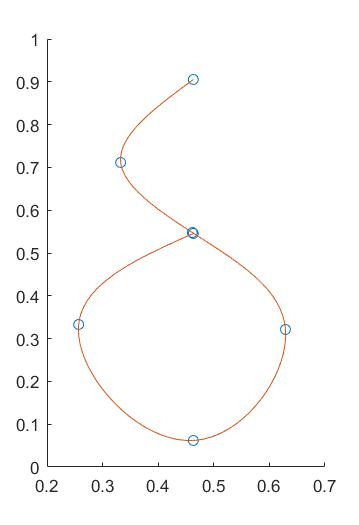
\includegraphics[width=.4\linewidth]{afbeeldingen/delta_result.jpg}
  \caption{delta}
\end{subfigure}%
\begin{subfigure}{.5\textwidth}
  \centering
  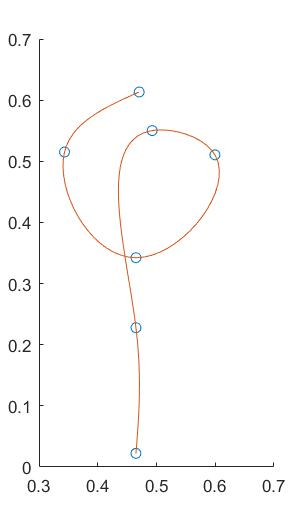
\includegraphics[width=.4\linewidth]{afbeeldingen/phi_result.jpg}
  \caption{phi}
\end{subfigure}
\caption{griekse letters benaderd door interpolerende, kubische splinecurven}
\label{fig:griekse_letters}
\end{figure}

In figuur \ref{fig:lalinea} zie je op dezelfde manier de splinevoorstelling van het mannetje van La Linea. Ook hier ziet men duidelijk dat knikken niet worden weergegeven. Dit is logisch aangezien dit een ander probleem is dan het opstellen van een natuurlijke, interpolerende, kubische splinecurve. Er zouden immers andere voorwaarden opgelegd worden aan de verschillende afgeleiden.

\begin{figure}[htb]
    \centering
    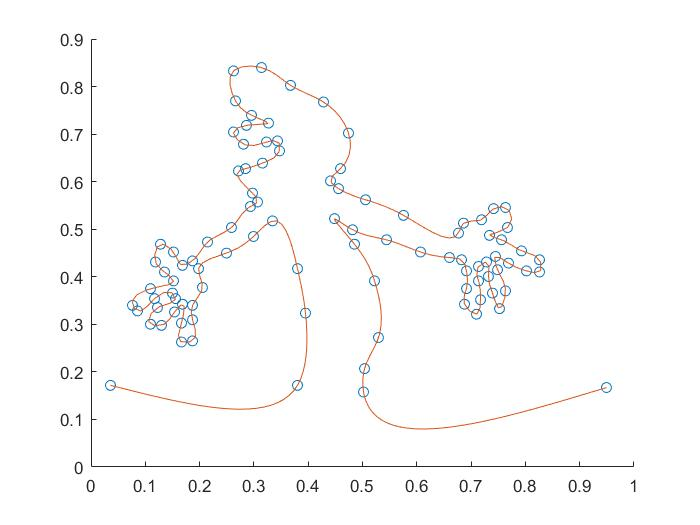
\includegraphics[width=0.7\textwidth]{lalinea_result.jpg}
    \caption{splinevoorstelling van het mannetje van La Linea}
    \label{fig:lalinea}
\end{figure}